%******************************************************************
%******************************************************************
\chapter {Introduction}
%******************************************************************
%******************************************************************


In this chapter we give a motivation for our work, discuss the possibilities of time-resolved X-ray imaging methods and arising problems for data analysis. The imaging principles and application fields are shortly described for radiography and tomography experiments. Further we give an introduction to optical flow methods and a general mathematical model behind their principle. We proceed with an overview of related work on the optical flow methods. In the end of the chapter we specify the aims of this work.



%--------------------------------------------------------
\section{Motivation}
%--------------------------------------------------------

%\subsection{Time-Resolved X-Ray Imaging}
%\label{time_resolved}

The discovery of physical phenomena such as X-rays, ultrasound, radioactivity, magnetic resonance, and the development of imaging instruments based on their principles, has revolutionized the fields of medical imaging and materials research.  Among other techniques, X-ray imaging is recognized as a genuine tool to image the internal structure of opaque objects, which is possible due to the penetration properties of X-ray radiation.
X-rays usually do not require special sample treatment and allow to use dedicated sample environments for \textit{in-situ} experiments. 
New methods emerged with the development of synchrotron radiation
X-ray sources. Modern synchrotron facilities, equipped with high-resolution detector systems provide intense radiation and high spatial resolution. This allows to investigate a broad spectrum of dynamical processes  in materials and biological samples.


Conducting an \textit{in-situ} experiment, triggering the process of interest, and then collecting time-lapsed data, enables to visualize and study dynamical phenomena. After the X-ray experiment is performed, all underlying events and internal changes are captured in a sequence of radiographic images or tomographic volumes. This makes time-resolved X-ray imaging a powerful tool that offers the exciting possibility to observe real-time dynamics and reveal internal structural information.


A vast variety of X-ray imaging methods, experiment types and sample forms give rise to a numerous challenges in the subsequent data analysis. Application examples of time-resolved X-ray imaging include evolution of morphological structures, monitoring of fabrication processes, investigation of materials under mechanical stress or heat treatment, velocimetry of liquid flows and diffusion processes, examination of living organisms and many other studies from various research fields. 

The common point of interest of these problems is the dynamics of a process. From the data processing perspective we can identify several topics of interest for time-resolved data analysis. First, it is \textit{motion analysis}, which includes the analysis of various qualitative and quantitative characteristics of the moving scene or objects, such as motion type, existence of sources and sinks, velocity or acceleration profiles. Another task is to perform the detection of objects by the analysis of their motion, the so-called \textit{motion-based segmentation}. The next typical task is \textit{object tracking}, which is a procedure for estimation of the trajectory of an object as it changes its position over time. To perform such a broad spectrum of data analysis tasks, a method capable of retrieving temporal changes and capturing dynamical information is required. In this work we present a general-purpose framework for time-resolved data analysis based on \textit{optical flow}. 
 

\textit{Optical flow} methods traditionally belong to the field of Computer Vision. A problem of finding correspondences between time-lapse images is useful for a variety of applications such as robot vision, tracking systems, video analysis and stereo reconstruction. The application of optical flow methods become increasingly important in other fields, such as medical imaging, materials research and life sciences. 
In this work we adapt \opticalflow methods to the task of time-resolved X-ray data analysis and show that these methods are well suited for a broad range of scientific problems. We restrict ourselves to a specific class of approaches that can be used to determine the optical flow, the so-called \textit{variational methods}. These methods are recognized among the currently most accurate, flexible and robust techniques for the \opticalflow computation \cite{Middl, Sun14}. 


%--------------------------------------------------------                
\section{Outline}
%--------------------------------------------------------
This work is organized in the following way.

In the beginning of Chapter 1 we shortly discuss the possibilities of time-resolved X-ray imaging methods and arising data analysis problems. X-ray imaging principles will be described shortly for radiography and tomography experiments. Additionally, we discuss their advantages and shortcoming with respect to time-resolved imaging. Further we give a short introduction to optical flow methods and describe the related work. In the end of the chapter we state the aims of this work.

Chapter 2 is dedicated to an extensive description and evaluation of \opticalflow methods. Quality and confidence measures for motion estimation are introduced.  We present different approaches for the construction of variational models and discuss how these techniques can be applied for particular types of X-ray data. We proceed with an extension of the devised 2D methods into a 3D model, which enables us to perform data analysis of tomographic data.  Next, we explain how a variational functional can be solved numerically using iterative methods. Furthermore, we discuss various computational aspects such as the coarse-to-fine strategy.

In Chapter 3 we consider important topics of data preprocessing and motion analysis. Several strategies will be presented to cope with the most important data challenges such as image noise filtering, correction of inhomogeneous brightness and enhancement of features contrast. The influence of the proposed filtering techniques on the performance of \opticalflow methods results will be discussed in detail. Then, we switch to the analysis of the computed flow field and temporal data.  We cover data analysis methods including advanced flow analysis, automated tracking,  motion-based segmentation, image registration and detection of temporal changes. All the presented techniques will be tested on synthetic data in the experimental part of the work (see Chapter \ref{experiments}) and employed in the part devoted to applications (see Chapter \ref{applications}).

In Chapter 4 we describe our computational framework. First, we present our software modules and describe their components and responsibilities. Then, we discuss an important topic of efficient and high performance computation of the \opticalflow. A number of optimization strategies will be presented. Next, we provide an efficient implementation of the \opticalflow algorithms on the GPU computing architecture. The last section of the chapter is dedicated to visualization methods. Here we present our own implementation of vector fields visualization, which allows for interactive inspection of the optical flow results.

%Moreover, we perform a brief overview of the existing data visualization and analysis software and provide a comparison of the their main features.

In Chapter 5 we perform  systematic numerical experiments on synthetic data, designed to test the performance of computational methods.  In the beginning of the chapter we provide a taxonomy of X-ray data. We present the quantitative evaluation of the performance, influence of preprocessing, modeling of noise and data outliers in dedicated sections. For all the experiments we outline important observations and draw the respective conclusions, which we summarize at the end of the chapter.

In Chapter 6 we apply our framework to various scientific examples from different research fields. These application examples include flow analysis and particle segmentation in semi-solid alloys, analysis of morphogenesis in living frog embryos, estimation of coalescence events and stability studies during the foaming process in various kinds of foams, and tracking of morphological dynamics in a living insect.
For each application we give a short description of a problem and specify our data analysis tasks. We evaluate the dataset according to our data taxonomy. Then we provide a detailed discussion on the choice of the appropriate data preprocessing  routines, selection of a suitable \opticalflow model and the selection of the specific data analysis technique, which will lead to the solution of the declared scientific aim.

In Chapter 7 we summarize the main results of our work and give our conclusions about the developed techniques. We also discuss a number of possible extensions and promising ideas which might further improve the results and extend our capabilities for analysis of challenging X-ray data.  




%--------------------------------------------------------
\section{X-ray Imaging}
%--------------------------------------------------------

\subsection{Introduction to X-ray Imaging}

X-rays were discovered by W. C. R\"ontgen on 8 November 1895 \cite{Roentgen1896}. In 1901 for this discovery and his investigations he obtained the first Nobel Prize in Physics. X-rays are electromagnetic radiation with a wavelength in the range of 0.01 to 10 nanometers, which corresponds to frequencies in the range $3 \times 10^{16}$ Hz to $3 \times 10^{19}$ Hz and energies in the range 100 eV to 100 keV. 

Due to their penetrating ability, hard X-rays (with photon energies between 10 - 100 keV) are an invaluable tool to image the internal structure of optically opaque objects. Already shortly after the discovery, X-ray imaging became widely used for medical applications, non-destructive testing and security systems. During propagation through the matter the intensity of X-rays is attenuated along their path of propagation. For 2D radiography imaging, the variations in thickness or properties of materials provide a contrast to resolve  different  structures. However, in this case one obtains only a projected image and loses any depth information due to superimposed structure details.

\textit{Computed tomography} (CT) overcomes this limitation and provides a three-dimensional information about the internal structure. To achieve this, a series of projections from different angles are acquired. Then, a reconstruction algorithm is used to yield a 3D digital representation of an object.  The mathematical foundations  for tomographic reconstruction were established by J. Radon in 1917 \cite{Radon17} and the CT technology was developed by G. Hounsfield and A. Cormack in 1960s-1970s.  Since then the computed tomography has revolutionized the fields of medical imaging and materials research.

\begin{figure*}[t]
  \centerline{
  %\mbox{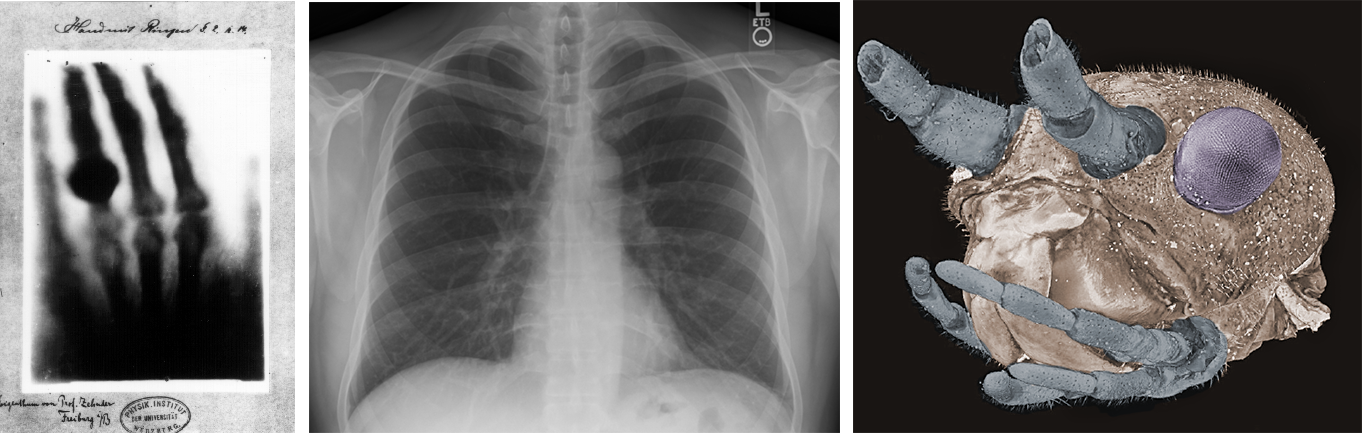
\includegraphics[scale=0.325]{figures/xrays_examples_all.png}}%
    \mbox{\includegraphicslabeledw[scale=0.32]{figures/xrays_hand.png}{a}}
    \mbox{\includegraphicslabeledw[scale=0.288]{figures/xrays_chest.png}{b}}
    \mbox{\includegraphicslabeledw[scale=0.368]{figures/xrays_insect2.png}{c}}
  }
  \caption[]{Evolution of X-ray imaging techniques. \textbf{(a)} First medical X-ray by Wilhelm R\"ontgen of his wife's hand. Image: Wikipedia, public domain. \textbf{(b)} X-ray radiography of a chest. Image: Wikipedia, public domain   \textbf{(c)} Volume rendering of the head of the stick insect \textit{Peruphasma schultei} imaged by a high resolution microtomography  \cite{vandeKamp13}.}
  \label{fig:xray_examples}
\end{figure*}

New methods and imaging techniques emerged with the development of \textit{synchrotron radiation}
sources. This radiation is generated using charged particle
accelerators.  Synchrotron radiation is emitted by the charged particles which are accelerated by magnetic fields on a circular trajectory in a storage ring. 

Modern 3rd-generation synchrotron radiation sources, equipped with high-resolution detector systems provide small beam size, high radiation intensity and high spatial resolution.
With the introduction of various X-ray optics the beam quality can be controlled, providing polychromatic or monochromatic radiation.
Synchrotron sources are expensive, not portable and usually are operated by large-scale facilities, which could limit a broad use of this technology. However, the unique quality of its probe make them a powerful tool for a wide range of X-ray experiments and applications.


\subsubsection*{X-ray Imaging Principles}
\label{xray_imaging_prnciples}

X-rays interact with matter either by \textit{photoelectric absorption} or \textit{scattering} (Compton and Rayleigh).  An absorption effect occurs when the X-ray photon is absorbed  in the course of liberating an electron from the inner shells of an atom. This contributes to the radiation dose defined as the amount of absorbed energy per unit of mass. This aspect is crucial for imaging of biological specimens. For a Compton scattering only a part of the X-ray photon  energy is used to free an electron  from an outer shell and the photon itself changes its direction, i.e. scatters \cite{Dougherty09}.
 
As a result of these interactions the intensity of the incoming beam is reduced. Various tissues or materials affect the changes in radiation intensity differently. In a homogeneous object this depends on its thickness $l$ along the direction of propagation and the attenuation coefficient $\mu$ of the material. The intensity $I$ of the incident X-ray beam after propagation through the sample of thickness $l$ is related to its initial intensity $I_0$ by the following expression:
$$I = I_0 e^{- \mu l},$$
which is known as a Beer - Lambert law.
    

%\change{From: Dougerty.
%Photoelectric absorption depends on the effective atomic number of the material, Zeff,
%and the x-ray energy, E, roughly as Zeff
%3/E3; and Compton scattering depends on the
%electron density of the material, ρelect, which varies roughly as Zeff, and the x-ray energy,
%as ρelect/E. Thus materials such as bone have a higher value of attenuation coefficient
%and attenuate x-rays more than soft tissues, as a consequence of their larger Zeff, and
%(photoelectric) absorption is the dominant interaction. Materials with a high effective
%atomic number, such as iodine (Zeff = 53) or barium (Zeff = 56), can be used to increase
%attenuation. They can be injected or swallowed to change the attenuation of soft tissues
%filled with the material compared to other soft tissues, and are known as contrast agents.
%For higher-energy x-rays, the overall attenuation is smaller with very much smaller
%photoelectric absorption and Compton scattering becoming dominant.}

Depending on the main effect of X-ray interaction with matter it is possible to classify  imaging techniques into \textit{absorption imaging} and \textit{phase-sensitive imaging}.
For the absorption imaging the contrast is produced by the attenuation of x-rays and is described as an amplitude modulation of the wave-field. In the case of  phase-sensitive imaging, contrast is governed by the
phase modulations due to the differences in spatial distribution of the refractive index.    
A number of phase sensitive imaging techniques might be used. A simple and popular method exploits the effect of propagation of the X-ray wave-field after its  interaction with the sample. Due to interference effects caused by the propagation,  the phase modulation can be reconstructed and visualized. For this technique a quantitative retrieval of the phase modulations is possible \cite{Cloetens99ab}, which allows to extract the real part of the refractive index in the interior of the investigated sample. 


%\subsubsection*{X-ray Sources Properties}
%X-ray source: flux, brilliance, coherence
%
%\change{From: Lukas. Important characteristic parameters of synchrotron sources are the source size and the
%brilliance [Rao93]. If the average electron velocity is defned parallel to y the brilliance
%is dened as (brightness/) where x and z are a measure of the source size in the
%x and z directions, respectively (i.e. FWHM of the spatial intensity distribution). The
%brightness is dened as the number of photons emitted per unit time into a unit solid
%angle and in a spectral bandwith = 10. }
%
%\change{From: Lukas. In the context of imaging applications, the low divergence of SR (especially of wigglers
%and undulators) allows one to place the object at a large distance from the source
%without losing a large portion of the emitted power. This is especially important for
%phase-contrast imaging (see Sect. 2.5.6): the high source-to-sample distances (and low
%source sizes compared to earlier generation synchrotron sources) enhance beam coherence
%signicantly. }


\subsubsection*{Beam Geometry}
Depending on the instrumental implementation of a X-ray source a number of different beam geometries are possible:

\begin{itemize}
\item \textit{Pencil beam}. The first X-ray source was implemented using a so-called pencil beam. For this geometry the cone of generated X-ray beams is filtered by a pinhole and, thus a point-like X-ray source is produced. A single detector is placed to the opposite side of the source to detect the X-rays.

\item \textit{Fan beam}. In this case the beam geometry is represented by a flat fan shape (divergent beam) and a detector system consists of an array of detector elements. Typically, the angle of beam divergence is small, as well as the size of the detection array.

\item \textit{Cone beam}. In this geometry the beam is a 3D cone with a wide angle of divergence and a large 2D detector is used. This technique is widely used in a laboratory-based X-ray setups. For this type of geometry the distance between the sample and the source is important, since it influences the object magnification in the detector plane.
Additionally, for image reconstruction algorithms the angular distribution of the incoming rays with respect to the rotation axis has to be taken into account \cite{Kak01}.

\item \textit{Parallel beam}.  The X-rays are coming parallel to each other and impinge on the sample perpendicular to its rotation axis. The 3D image reconstruction procedure for this type of geometry is the simplest and can be realized in an efficient way \cite{Kak01}.
\end{itemize}

%\begin{figure*}[t]
%  \centerline{
%    \mbox{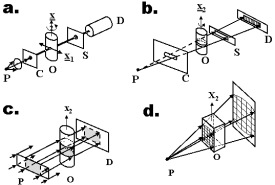
\includegraphics[scale=0.75]{figures/beam_geometry.png}}
%  }
%  \caption[]{Fast radiography of a feeding cockroach \textit{Periplaneta americana}. \textbf{Left:} Fist frame of the  radiographic sequence. (The background is removed and contrast is adjusted). \textbf{Right:} Computed motion field.  Color shows particular movement direction.}
%  \label{fig:beam_geometry}
%\end{figure*}

 
 In the current work all experimental results presented in the application sections are obtained using the parallel beam geometry. The most important aspect related to data analysis is the quality of 3D reconstructed images. Each beam geometry is associated with its own set of reconstruction artifacts \cite{Buzug08}. Therefore, the beam geometry, experimental parameters and the reconstruction algorithm strongly influence the later stages of data processing and analysis. We discuss these aspects in the Section \ref{computed_tomography} devoted to tomographic reconstruction.    




\subsubsection*{Detector System}

After the interaction with an object and propagation to the detector plane, X-rays are registered by a detector system. Two distinct classes of detectors are used in synchrotron radiation imaging \cite{Gruner01}:
\begin{itemize}
  \item \textit{Direct photon detectors}.  For this type of detector systems X-ray photons are converted directly into an electric charge. 
  \item \textit{Indirect detectors}. For the indirect detection system the incident photons first strike a material layer, called scintillator, which converts X-ray photons into visible-light photons. These photons are then detected by a visible-light detector.  
\end{itemize}

For each detector system a number of technologies are available, such as charge-coupled devices (CCD) and complementary metal-oxide-semiconductor (CMOS) cameras.
A substantial advantage of the indirect detector system is that a wide range of commercially available high-performance, visible-light cameras is available. With the recent developments such cameras can achieve a very high spatial resolution (down to 1.0 $\mu m$) and ultra fast data acquisition rates (up to 100.000 frames per second) \cite{Rack10}.    


\subsubsection*{Digital Image}
\label{digital_image}

\textit{Spatial resolution} is the capability of an image to represent object details. It can be characterized as the minimum separation distance of nearby features of the object which can still be recognized on the image as different structures.  In general, the spatial resolution of a digital image depends on the resolution of the imaging system described by its point spread function (PSF) and the pixel size of the detector system \cite{Dougherty09}.
The \textit{pixel size} of the digital detector is determined by the sampling frequency used to digitize the image signal and by the physical size and separation of the array elements within a 2D detector. Increasing the pixel size reduces the effective resolution, but can lead to the increased signal sensitivity.
The \textit{point spread function} describes the response of the imaging system given a point source or a point object. The width of the PSF function determines the size of the smallest detail that can be resolved. According to the sampling theorem \cite{Nyquist28}, the pixel size should be less or equal half the width of the point spread function in order to correctly sample an analog signal. For smaller pixel sizes the PSF spreads to several pixel locations and the resolution is reduced.

%\change{From: Lukas. The detective quantum e±ciency of a detector system is de¯ned by the signal-to-noise
%ratios (SNR) at the input and the output according to: (FORMULA) where at the input for photons with Poisson statistics (FORMULA)
%can be assumed. For an ideal detector the DQE equals 1 whereas real detectors show
%a DQE smaller than 1. Therefore the latter require increasingly better input statistics
%(e.g. by increase of the exposure time) the worse their DQE is.}



Another important characteristics of the digital image is the \textit{brightness resolution}. In a digital image differences between structures are represented by variations in brightness values. In X-ray imaging, these variations are determined by or related to the physical properties of a sample, such as sample thickness, material density and chemical composition. The aim of an imaging process is to distinguish between various parts of the sample, which differ in their structure or material composition. Ideally, this should also be valid if both materials differ from each other only slightly. To achieve this a detector system with a good brightness resolution should be used. This property is also called the \textit{dynamic range} of the detector system. The range of brightness variations which is recorded depends also on the number of bits used for quantization procedure (converting the analog signal to digital).  Most modern camera systems allow to record images in 12, 16 or 32-bit value formats. We discuss further aspects related to the brightness resolution in the Section \ref{contrast_adjustment}, which is dedicated to preprocessing of low-contrast image data.

\subsection{Experimental Methods}

In this section we briefly describe two imaging techniques, which will be employed in this work to acquire a sequence of time-lapsed X-ray images - radiography and tomography. For both experimental techniques we describe the advantages and shortcomings of its application with respect to its ability to capture spatio-temporal information. Moreover, we introduce typical challenges that arise during data processing and optical flow computation.

\subsubsection{Radiography}

\textit{Radiography} is a simple, yet powerful technique to visualize internal structures of a sample. For this purpose a sample is placed in the beam and properly aligned using manipulation devices (e.g. translation stages), so the optimal position in the field of view is achieved. As soon as the process of interest is triggered, a high speed camera records time-lapse projection images, called "radiograms". Many instrumental modifications for the radiography experiment setup are possible. They include the choice of the X-ray beam properties, positioning devices, source-to-sample and sample-to-detector distances, detector optics and the choice of digital camera or sensor.

We now describe a number of characteristic properties associated with the radiography technique.
Among the advantages of this method are:
 \begin{itemize}
  \item   High spatio-temporal resolution: Spatial resolution down to the micrometer scale and temporal resolution down to the microsecond range are achievable with modern detector systems \cite{Rack10}.
  %\item   Temporal resolution depends on the motion of the sample and the frame rate of a detector system. Assuming that the sample movement cannot be controlled, in order to improve temporal resolution, the acquisition frame rate should be increased. Having only one parameters to adjust, makes it is easier to perform an \textit{in-situ} or \textit{in-vivo} experiment.
  \item In most cases no complicated alignment of the sample is needed  - the sample is simply placed in the field of view of the detector system.
  \item Since the sample stage does not move during the data acquisition, the usage of complex or bulk sample environments is possible (e.g. furnace, high-pressure chamber, etc).
\end{itemize}
However, there are also a number of major drawbacks, that limit applicability of the radiography:
 \begin{itemize}
    \item   The main drawback of the radiography technique originates from the projection of 3D structures on a single 2D image plane. As a result, any depth information about internal 3D structures is inevitably lost.
    \item   For data processing methods, including correspondence problems (e.g. optical flow, object recognition), the superposition of 3D structures into a 2D plane imposes a critical challenge - the underlying assumptions on data constancy and the affine transformation model are no longer valid. For example, the change in orientation of the object in 3D space causes a redistribution of the projected thickness on the image plane. Thus, no reasonable assumption about the image data can be enforced. In some situations the movement in 3D space does not cause a change in the distribution of grey values in the projected 2D image. One example is  an object, which undergoes a translational movement perpendicular to the projected plane and the parallel beam geometry is used.         
 \end{itemize}


\begin{figure*}[ht]
  \centerline{
    \mbox{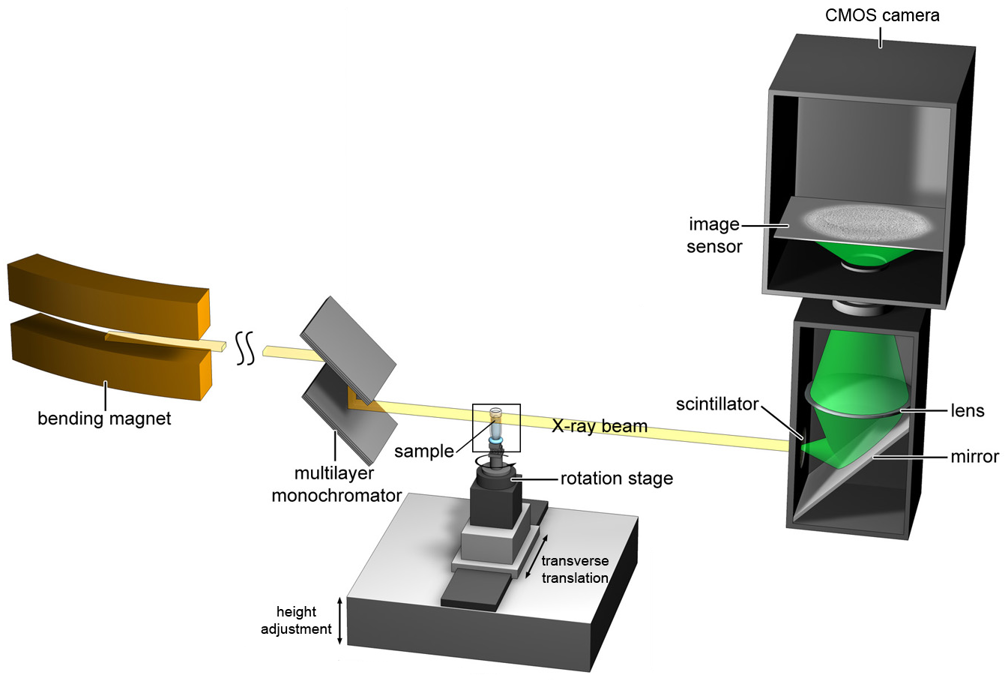
\includegraphics[scale= 0.30]{figures/tomo_setup.png}}
  }
  \caption{Experimental setup for propagation-based phase-contrast X-ray
microtomography. A photon beam is generated by the synchrotron. After the beam is shaped and filtered by the monochromator, the X-rays propagate over a large distance
to interact with the sample mounted on a rotation stage for
tomographic data acquisition. The 2D detector system consists of a scintillator, which converts X-rays into a visible light, a mirror, a lens and a CMOS digital camera. Image: \cite{Nature13} }
  \label{fig:tomo_setup}
\end{figure*}



\subsubsection{Computed Tomography}
\label{computed_tomography}

The previously described radiographic technique suffers from a major drawback - it only produces a projection of three-dimensional objects on the 2D detector plane. As a result the structures are superimposed with each other, which complicates their identification and analysis. Computed Tomography (CT) is a technique which has been developed to overcome this limitation. It provides a three-dimensional information about the inner structures of an object.
This technique consists of two stages. First, a series of radiographic projections from different directions are taken.
Then, a dedicated  algorithm is used to reconstruct a 3D volumetric image. 
The task for tomographic reconstruction is to perform the retrieval of the unknown object function from a series of its Radon transformations taken from different angles \cite{Kak01}.
There are two distinct classes of tomographic reconstructions:
\begin{itemize}
\item \textit{Analytical methods} are based on reconstruction steps using the Fourier transformation \cite{Kak01}. It is important to note, that such methods yield an exact solution of the inverse problem if a number of requirements are fulfilled. For large tomographic datasets these methods a preferred since they are typically less computationally demanding. Moreover, they are also less sensitive to noise and small data artifacts, thus producing more accurate results. One popular choice for such type of techniques is the \textit{filtered back-projection} (FBP) \cite{Kak01}.

\item \textit{Algebraic methods} represent an object as an array of unknown coefficients and model a ray transmission through the object as a mathematical function of these coefficients. Then a system of algebraic equations is solved to estimate the object. Usually this class of reconstruction methods is used if the requirements for the analytical methods are not satisfied. For instance, if the number of angular projections is insufficient. Or if the beam geometry and tomographic acquisition is hard to be modeled analytically, e.g. for diffraction tomography.         
\end{itemize}


A typical tomography setup is shown in Figure \ref{fig:tomo_setup}. Here we list advantages and drawbacks of the computed tomography technique.  Among the advantages are:
 \begin{itemize}
  \item   Computed tomography provides a 3D structural information about a sample. 
  \item   For the computation of optical flow having a 3D representation of a  scene and its objects means that there are no occlusions between different structures (as it happens for 2D images). This highly influence the accuracy of motion estimation and leads to better results.
\end{itemize}
Nevertheless, there are also a number of limitations:
 \begin{itemize}
  \item   The need of tomographic acquisition, which involves imaging of an object from multiple directions, can limit temporal resolution. This is especially critical for imaging rapid dynamical processes. 
  \item   The rotation of the sample on the tomographic stage could also restrain the use of sample environments (wiring, bulky instrumentation, etc), which cannot be rotated freely around an axis. 
  \item   To obtain tomographic volumes of a high quality, a large number of radiographic projections is required. Depending on the sample and properties of the X-ray radiation, it may result in a high dose deposition. This aspect is crucial for imaging living specimens and can limit the applicability of X-ray computed tomography.   
  \item Depending on the number of projections, image quality and specific image artifacts could appear and degrade the resulting 3D data. Compared to such image characteristics, such as noise and low contrast, these artifacts are difficult to correct. The presence of reconstruction artifacts significantly reduces the performance of optical flow methods. 
\end{itemize}



%\subsubsection{[OPTIONAL] Laminography}
%
%\begin{itemize}
%	\item   Method
%  \item   Setup. Setup scheme
%  \item   Advantages and shortcomings: Similar to CT. What else?
%  \item Short experiment example (Inspection Flip-chip devices)
%	\item References
%\end{itemize}



%--------------------------------------------------------
\section{Variational Optical Flow}
%--------------------------------------------------------

\textit{Optical flow} is one of the major problems in \textit{Computer Vision}.  Given a sequence of images the aim is to determine the correspondences between them. A method to find the displacement field which maps all image points from the first frame to their new locations within the second frame is called \textit{optical flow}. Following a formulation from the seminal work of Horn and Schunck \cite{HornSchunck81}, the motion field is the 2D projection of the actual 3D motion of objects and scene, where the \opticalflow is the \textit{apparent} motion of the brightness patterns depicted on the image.   In our work we extend the definition of optical flow as an actual 3D motion of internal structures when applied to 3D tomographic volumes.

\Opticalflow is useful for a variety of different applications such as robot vision, driver assistant systems, object tracking and stereo reconstruction, video analysis and processing \cite{Wolf96, Sudhir96, Kastrinaki03, Hu04}.    In this work we employ \opticalflow methods to perform data analysis and investigate of a wide range of applications related to the field of X-ray imaging. One example is given in Figure \ref{fig:example_feeding_insect}, where \opticalflow is used to capture real-time movements of the feeding cockroach.

\begin{figure*}[ht]
  \centerline{
    \mbox{\includegraphicslabeledb[scale=0.33]{figures/bug_full_original_enh.png}{a}}
    \mbox{\includegraphicslabeledb[scale=0.33]{figures/bug_full_colors.png}{b}}
    \mbox{\includegraphicslabeledb[scale=0.5]{figures/color_code_inverted.png}{c}}
  }
  \caption[]{Fast radiography of the feeding cockroach \textit{Periplaneta americana}. \textbf{(a)} First frame of the  radiographic sequence (the background is removed and contrast is adjusted). \textbf{(b)} Computed flow field, which captures the movements of the insect. \textbf{(c)}  Color coding: color represents direction and its brightness represents flow magnitude.}
  \label{fig:example_feeding_insect}
\end{figure*}


\subsection{Related Work}

The research on \opticalflow estimation advances is rapidly. The methods become more accurate, robust with respect to challenging data and flexible to model various scene and motion scenarios. In the scope of this work we restrict ourselves to a specific class of approaches used to determine the optical flow, so-called \textit{variational methods}. These methods are recognized as one of the most accurate and best understood techniques for the \opticalflow computation \cite{Middl, Sun14}. 

Recently a number of important contributions to the field of \opticalflow estimation were made. In the work of Bruhn \cite{BruhnThesis} a systematic taxonomy and quantitative evaluation of variational \opticalflow methods was presented. A common notation as well as an extensive list of available models allows to construct an optical flow framework, suitable for a wide range of applications. 
Development of a novel database for the evaluation of optical flow techniques has led to rapid improvements and understanding of optical flow methods \cite{Middl} . 
A vast amount of literature on motion estimation techniques propose sophisticated models and multiple features. This  makes it hard to evaluate the performance of the individual components. In Refs. \cite{Sun10, Sun14} the authors provide an overview over current state-of-the-art \opticalflow methods and reveal the "secrets" behind the most successful models.
Recently, some of the authors reported that even the most advanced approaches yield poor results on a challenging real-life data. This highlights the importance of work on  robust optical flow methods designed for a particular task or application. A number of application specific optical flow evaluation databases has already emerged \cite{Adato07, Geiger12}.

Many of the today's state-of-the-art variational \opticalflow methods still resemble the original
formulation by Horn and Schunck \cite{HornSchunck81}. This model combines a \textit{data term} that imposes constraints on image features which should be matched and a \textit{smoothness term} which regulates the properties of the flow field. A global energy functional containing both constraints is then minimized to find the solution. In this section we describe important work related to the modeling of data and smoothness assumptions, as well as the optimization procedure.  We also give a short outlook of works where optical flow methods has been applied.

There are many approaches and interesting concepts which go beyond the scope of this work. For example, we exclude the discussion of photometric data terms constancy assumption based on color information \cite{Mileva07},  motion with transparency or layered models \cite{Jepson93, Wang93, Ju96},  incorporation of feature descriptors (i.e. SIFT) to refine motion estimation during coarse-to-fine strategy \cite{Xu10},  combination of optical flow estimation and image segmentation \cite{Black96b, Zitnick05, Xu08}, or the use of non-convex optimization strategies.  We will restrict ourselves only to those approaches which are suitable for the application on the X-ray image data and can be incorporated to the variational framework. 

\subsubsection{Data Assumptions}

In the literature, there are two major directions for the formulation of data constraints: design of robust data terms, which improve the performance on problematic image data and incorporation of additional information to model various aspects, such as illumination changes and different motion models. 
The first approach for the robust data term was proposed in the work of Black and Anandan \cite{Black91, Black96}, where the quadratic function of the original Horn and Schunck method was replaced by a non-quadratic variant. The robust modeling of data constraints become an important factor in the construction of accurate optical flow methods \cite{Brox04, Lempitsky08, Xu10, Middl, Sun14}. 
In order to handle varying illumination conditions,  higher order constancy assumptions \cite{Schnorr93, Schnorr94,  Brox04, Papenberg06, HarmonyFlow} or special image filtering are proposed \cite{Mileva07, Wedel09, HarmonyFlow}. To improve the performance of data constraints for noisy images some of the authors suggested a local-global data term \cite{Bruhn02, Bruhn05a}, which takes into account the information around a local region.  

\subsubsection{Regularization}

The regularization of flow fields involves two main aspects: discontinuity preserving motion estimation and incorporation of temporal information.
The first approach to use adaptive smoothness was proposed by Nagel et al. \cite{Nagel83, Nagel86}. This idea has been developed in a number of approaches which assume image-driven \cite{Schnorr93, Alvarez99} or flow-driven smoothness \cite{Shulman89, Schnorr94}.  In Ref. \cite{Sun08} the authors combined the advantages of both methods to obtain precise motion discontinuities and avoid oversegmentation problems. In their work the smoothness direction is adjusted to image edges and smoothing amount to the flow gradient. In Ref. \cite{HarmonyFlow} the authors generalized this idea to obtain a \textit{complementary smoothness} term.  Such approach regulates the smoothness direction according to the data constraint, instead of image edges.

The idea to assume the smoothness also in temporal direction was first investigated  by \cite{Murray87} and extended for continuous models in \cite{Nagel90}. A discontinuity-preserving spatio-temporal smoothness was proposed in \cite{Weickert2001b} and used for a number of highly accurate \opticalflow models \cite{Brox04, HarmonyFlow, Volz11}.

\subsubsection{Solution}

To find a solution of variational methods in the presence of large displacements it is common to use a coarse-to-fine strategy \cite{Black96, Memin98, Brox04, Xu10}. For the construction of image pyramids and in order to perform image warping a bicubic interpolation is commonly used \cite{Sun10}.
In order to represent image gradients a second order derivatives, as well as temporal averaging are among good practices \cite{Wedel09, Sun14, HarmonyFlow}. A number of efficient computation models were proposed, such as multigrid methods \cite{Bruhn05, Bruhn06b}. Furthermore, a popular trend is a fast implementation of variational methods using graphical processing units (GPU) \cite{Wedel09, Gwosdek12, Bao14}.


\subsubsection{Applications}


Optical flow methods are widely used in the native field of Computer Vision, for such applications as video surveillance and analysis \cite{Kastrinaki03, Hu04}, video compression \cite{Wolf96} and video annotation \cite{Sudhir96}. Recently, the usage of optical flow methods become important for data analysis in the fields of biological imaging and life sciences, as well as in other research fields. Examples include: zebrafish development \cite{Amat13}, monitoring of plant growth \cite{Barron97}, in-vivo blood flow measurements \cite{Vennemann07}, modeling and correction of respiratory motion \cite{McClelland13} and analysis of cardiac images \cite{Xu10b}.


Various parts of the current work were presented in publications, dedicated to  X-ray imaging \cite{Baumbach09, Rack10, Altapova12}, applied for \textit{in-situ} studies of advanced materials \cite{Zabler10, Myagotin12, Zabler13} and for \textit{in-vivo} investigation of various biological questions \cite{Betz08, Nature13, van13, Moosmann14, dosSantosRolo14}. 


\subsection{General Model}
\label{general_model}

A general model for variational methods was proposed by Horn and Schunck in 1981 \cite{HornSchunck81}. This technique determines the unknown displacement field as a minimal solution of the  \textit{energy functional}. In general, such energy-based formulations are composed of two parts: a data term which assumes constancy of specific image features, and a smoothness term which regularizes the spatial variation of the flow field.
 
The classical \opticalflow approach of Horn and Schunck consists of a \textit{brightness constancy} assumption and a \textit{homogeneous} smoothness term. The first constraint states that after the displacement the  brightness value remains constant and the second constraint assumes that the motion field varies smoothly in all directions.

In order to formulate the \opticalflow model we consider a time-lapse sequence of images $I(x,y,t)$, where $(x,y)$ are the pixel coordinates within an image domain $ \Omega_{2} \subset     \mathbf{R}^2$ and $t$ denotes time frame. Then, the brightness constancy assumption can be expressed by:
\begin{equation}
	I(x+u(x,y), y+v(x,y), t+1) = I(x,y,t),
	\label{eq:brightness}		
\end{equation}
where ($u(x,y),v(x,y)$) is the displacement field from frame $t$ to $t+1$. To simplify the formulation of model assumptions, we will use the short notation $u, v$ for the displacement field components  instead of $u(x,y),v(x,y)$.
Assuming that the displacement components are small and changing continuously, we can approximate the non-linear equation (\ref{eq:brightness})  using a first order Taylor expansion. We obtain the so-called \textit{ linearized optical flow constraint}:
\begin{equation}
	I_{x}u + I_{y}v +I_{t} = 0.
\end{equation}

The \opticalflow cannot be  uniquely computed at a single point since the displacement is given by two components, while the change in image brightness provides only one constraint. In the literature this is known as the \textit{aperture problem} \cite{Bertero88}. There are two different cases of this issue. If only one component of the image gradient can be computed, it is possible to determine the flow component parallel to the direction of image gradient, so-called \textit{normal flow}.
In the second case, in homogeneous image regions the brightness gradient vanishes completely, so no appropriate correspondence can be found. 

To overcome this problem, the method proposed by Horn and Schunck introduces an additional constraint which assumes the spatial smoothness of the flow field. Such constraint can be expressed by penalizing the spatial flow gradients, given by $\nabla_{2}u$ and $\nabla_{2}v$.
Both, the brightness constraint and the smoothness constraint can be integrated in the energy functional to obtain the classical Horn and Schunck method:

\begin{equation}
E_{\text{HS}}(u,v) = \int_{\Omega_{2}}{(I_{x}u + I_{y}v +I_{t})^2 + \alpha (|\nabla_{2}u|^2 + |\nabla_{2}v|^2) \text{d}x \text{d}y},
\end{equation}
where $|f| = \sqrt{f^2_x + f^2_y}$ is the magnitude and $\nabla_2 = (\partial_{x}, \partial_{y})$ denotes the spatial gradient. The parameter $\alpha$ is called \textit{regularization} or \textit{smoothness parameter} and controls the amount of required smoothness of the resulting flow field. 

The variational \opticalflow methods based on the Horn and Schunck model can be written in a more general form:

%$$E(u,v) = \int_{\Omega_{2}}{D(I,u,v) + \alpha \: S(I,u,v) dx dy},$$
$$E_{\text{general}} = \int_{\Omega_2}{(D(I, u,v) + \alpha  \: S(I, u,v)) \: \text{d}x \text{d}y},$$
where $D(I,u,v)$ imposes constraints on image features which should be matched and $S(I, u,v)$ regulates the smoothness properties of the flow field. Both parts of this general \opticalflow framework can be customized and adapted for the specific data properties and motion models. In Chapter \ref{optical_flow_methods} we present different approaches to construct accurate and robust variational \opticalflow models and discuss how these techniques could be applied for the particular task of X-ray data analysis.

In order to find the solution of the \opticalflow problem we are interested to have energy functionals which are \textit{convex}. For such functionals a \textit{unique solution} exists and it can be found using \textit{globally convergent} algorithms. In contrast, for non-convex approaches \textit{multiple local minima} can be present and optimization algorithms may suffer from getting trapped in local minima, thus providing inaccurate results. For the Horn and Schunck method linearization of the brightness constraint must be performed in order to obtain a convex functional. Such linearization step does not affect the accuracy of the result as long as only small displacements for the scene are considered. In order to cope with large displacements linearization procedure cannot be applied and the original non-linear variant of the data term must be used. In Section \ref{large_displacements} we will introduce a \textit{coarse-to-fine strategy} based on the theory of warping which allows to solve non-convex energy functionals for our problem.


 
%--------------------------------------------------------
\section{Aims of the Work}
%--------------------------------------------------------

As it was discussed in the introductory section, time-resolved X-ray imaging methods provide a wide range of possibilities for the research of dynamical processes. 
It is a challenging task, however, and involves many steps to get from the initial idea of the experiment to the final scientific result. 
After an experimental setup is prepared and carefully adjusted, the original raw data is recorded by a detector system.  The acquired data have to be inspected and evaluated to ensure that the desired image quality is achieved and the events of interest are captured.
At this step important adjustments could be introduced to improve the results. The raw experimental data coming from the detector system is usually not suited for the immediate analysis, since images often contain artifacts.  Thus, an artifact correction and data enhancement procedure is desirable. The quality of time-resolved X-ray data is immensely diverse. Data related properties, such as image resolution, signal-to-noise ratio, features contrast and underlying motion model, influence the performance of data processing routines. To automatically capture the dynamics of a process an appropriate computation algorithm should be employed.  In this work we use \textit{variational optical flow} as the core method to extract temporal information. 
%An overview of a typical experiment workflow is presented in Figure \ref{fig:pipeline_scheme}.   
%\begin{figure*}[ht]
%  \centerline{
%    \mbox{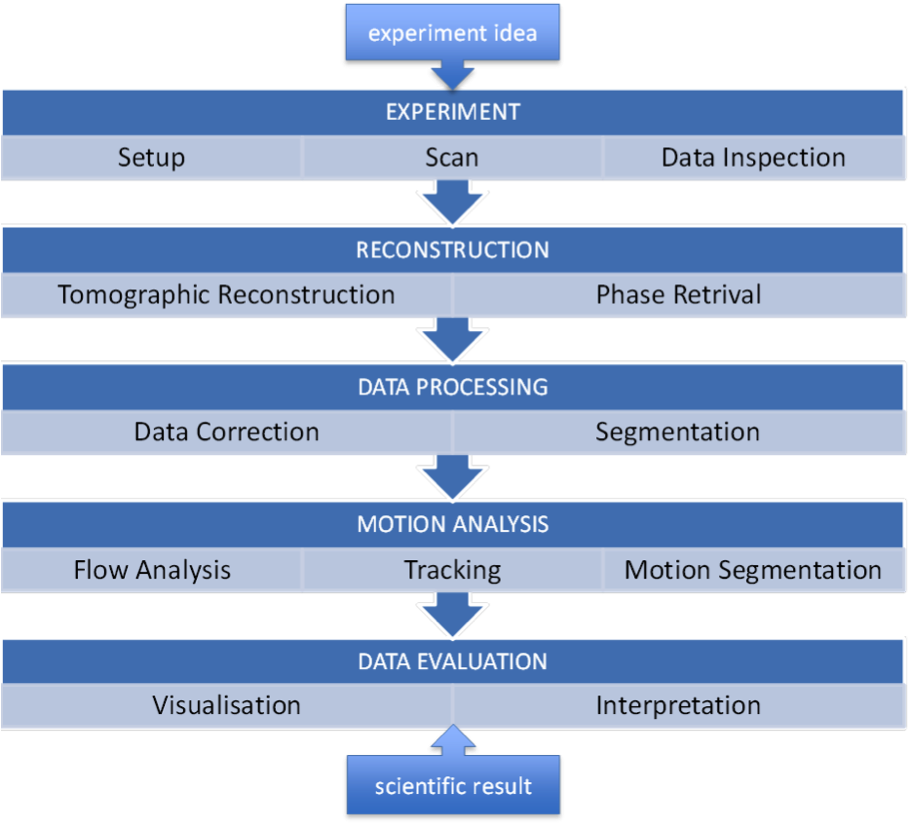
\includegraphics[scale=0.75]{figures/pipeline_scheme.png}}
%  }
%  \caption[]{\todo{Change} A general workflow for  time-resolved X-ray data analysis.}
%  \label{fig:pipeline_scheme}
%\end{figure*}
      
The main goal of our work is to cover, investigate and implement all the aspects that are important for automated analysis of time-resolved X-ray data. To achieve this we proceed with the following steps:
        
\begin{itemize}
    \item provide a detailed classification of X-ray data, including the description of image quality, motion types and features of interest. This taxonomy should serve as a reference point for the development of image preprocessing, data analysis and motion estimation procedures
    
	\item develop image preprocessing methods to enhance the original (raw) X-ray data
	
	\item perform systematic evaluation of state-of-the-art \opticalflow techniques, make quantitative analysis of their components and choose the most robust and accurate approaches
	
	\item introduce a flexible framework based on variational \opticalflow methods to extract dynamical information from time-lapsed datasets
	
	\item provide automated confidence measures to ensure the reliability of motion estimation. Such measures should also assist with the automated optimization of model parameters
	
	\item develop an extensive data analysis toolkit including automated tracking, flow analysis, motion-based segmentation, image registration and detection of temporal changes
	
	\item implement the developed techniques for 4D data (3D + time) to enable analysis of tomographic data
	
	\item provide an efficient implementation of optical flow methods using advanced numerical schemes and computations on graphics processing units (GPUs). Thereby, the processing of a vast amount X-ray data - long image sequences and large tomographic volumes - becomes feasible 
	
	\item apply the devised optical flow and data analysis techniques to investigate a number of scientific problems from various research fields 
\end{itemize}

All the aforementioned topics are essential for the subject of this thesis, therefore we consider them as a complete framework. However, some parts of this work are also useful as isolated topics.  As an example - in Section \ref{data_taxonomy} we provide an approach for qualitative data taxonomy and in Section \ref{data_preprocessing}  we present image processing routines to enhance the original X-ray data. These steps are general for various data analysis problems that are not related to analysis of dynamics (e.g. image segmentation). The variational \opticalflow methods which we use in this work could be substituted by any other technique solving the same class of problems, i.e. finding correspondences between time-lapse images. Therefore, the information presented in other parts, such as in the chapters dedicated to data analysis or applications are still valuable. The current work is interdisciplinary and closely related to the fields of Computer Science, X-ray imaging, Material and Life Sciences.

 




